\documentclass[11pt,a4paper]{article}

\usepackage[utf8]{inputenc}
\usepackage[T1]{fontenc}
\usepackage{lmodern}
\usepackage[margin=2.5cm]{geometry}
\usepackage{graphicx}
\usepackage{float}
\usepackage{booktabs}
\usepackage{tabularx}
\usepackage{fancyhdr}
\usepackage[hidelinks]{hyperref}

\newcommand{\product}{AI Models Comparator}
\newcommand{\team}{Vivien Gruel \\ Noé Wales \\ Valentin Gempp \\ Maxence Tessier}

\pagestyle{fancy}
\fancyhf{}
\fancyhead[L]{\product}
\fancyhead[R]{Software Requirements Specification}
\fancyfoot[C]{\thepage}

\begin{document}

\begin{titlepage}
  \centering
  \vspace*{4cm}
  {\Huge\bfseries \MakeUppercase{\product}\par}
  \vspace{1.5cm}
  {\LARGE Software Requirements Specification (SRS)\par}
  \vspace{4cm}
  {\large Software Engineering -- A4 -- 2026-2027\par}
  \vspace{1cm}
  {\large \team\par}
  \vfill
\end{titlepage}

\tableofcontents
\newpage

\section{Introduction}

\subsection{Purpose}

This document describes the functional and non-functional requirements of the \product{}. It explains \textbf{what} the system must do. It is written for the developers, the testers and the TD instructor, so that everybody has the same understanding of the project.

\subsection{Scope}

The \product{} is a web application that ranks AI models in two ways: with benchmark scores collected from external websites, and with the up and down votes of the users. Each model has its own page with its scores, its rankings and a comment feed. The website also shows news about new AI models. Administrators can moderate comments and users.

\subsection{Definitions, Acronyms, and Abbreviations}

\begin{itemize}
  \item \textbf{AI model / LLM:} a Large Language Model, for example GPT-5 or Claude.
  \item \textbf{Lab:} the company that created a model (for example OpenAI, Anthropic, Meta).
  \item \textbf{Benchmark:} a standard test used to measure the performance of a model (for example GPQA or MMLU-Pro).
  \item \textbf{Community score:} percentage of up votes that a model received.
  \item \textbf{Benchmark score:} average of the benchmark results of a model.
  \item \textbf{Slug:} a short text used in the URL of a model (for example \texttt{gpt-4o-2024-08-06}).
  \item \textbf{SPA:} Single Page Application.
  \item \textbf{API:} Application Programming Interface.
  \item \textbf{GDPR:} General Data Protection Regulation.
\end{itemize}

\subsection{References}

\begin{itemize}
  \item Business Requirements Document (BRD) of the \product{}.
  \item IEEE 830 / ISO/IEC/IEEE 29148 for requirements specification.
  \item SHMS SRS template given in the course.
\end{itemize}

\subsection{Document Overview}

Section 2 gives a general description of the product. Section 3 lists the functional and non-functional requirements. Section 4 describes the main use cases. Section 5 contains the UML diagrams. Section 6 describes the external interfaces and Section 7 the other requirements.

\section{General Description}

\subsection{Product Perspective}

The \product{} is a new, independent web application. It has a React frontend and a Node.js/Express backend with a PostgreSQL database. It depends on external websites for the benchmark scores and the AI news. These data are imported automatically by the backend and stored in the database, so the users never call the external websites directly.

\subsection{Product Features}

\begin{itemize}
  \item \textbf{Model catalogue:} all models grouped by lab.
  \item \textbf{Model page:} details, benchmark scores, rankings, votes and comments of one model.
  \item \textbf{Benchmark ranking:} ranking based on the benchmark scores.
  \item \textbf{Community ranking:} ranking based on the up and down votes.
  \item \textbf{Comments:} one comment feed for each model.
  \item \textbf{AI news:} list of news about AI models.
  \item \textbf{Accounts:} sign up, log in, log out, delete account.
  \item \textbf{Administration:} moderation of comments and users, status of the imports.
\end{itemize}

\subsection{User Characteristics}

\begin{itemize}
  \item \textbf{Visitor:} any person on the website without an account. Can read everything but cannot vote or comment.
  \item \textbf{Registered user:} a visitor with an account. Can vote, comment, and delete their own comments and account. Usually developers, students or AI fans.
  \item \textbf{Administrator:} a registered user with the ADMIN role. Can moderate all comments and users.
\end{itemize}

\subsection{General Constraints}

\begin{itemize}
  \item The frontend must be developed with React and the backend with Node.js (course requirement).
  \item The system must respect the GDPR.
  \item The system must respect the terms of use of the external data sources.
  \item The project must be finished during the sprints of the course, by a team of four students.
\end{itemize}

\subsection{Assumptions and Dependencies}

\begin{itemize}
  \item At least one external website gives benchmark scores with an API or a downloadable file.
  \item At least one free RSS feed or API gives news about AI models.
  \item Users have a recent web browser and an internet connection.
\end{itemize}

\section{Specific Requirements}

\subsection{Functional Requirements}

\subsubsection{Model Catalogue}

\begin{itemize}
  \item \textbf{FR-1.1:} The system must display all the labs in alphabetical order, each with its logo and name.
  \item \textbf{FR-1.2:} Under each lab, the system must display the names of its models in alphabetical order.
  \item \textbf{FR-1.3:} When the user clicks on a model, the system must open the model page at \texttt{/models/\{slug\}}.
  \item \textbf{FR-1.4:} The model page must show the name, the lab, the release date, the two ranks, the table of benchmark scores (benchmark, score, source), the community score with the number of votes, and the comment feed.
  \item \textbf{FR-1.5:} If the slug does not exist, the system must display a ``Model not found'' page (404).
\end{itemize}

\subsubsection{Benchmark Ranking}

\begin{itemize}
  \item \textbf{FR-2.1:} The system must import benchmark scores automatically every 24 hours.
  \item \textbf{FR-2.2:} The system must only keep benchmarks expressed as a percentage (0 to 100).
  \item \textbf{FR-2.3:} The benchmark score of a model is the average of all its benchmark results.
  \item \textbf{FR-2.4:} A model is in the benchmark ranking only if it has at least 3 benchmark results. Otherwise, it is shown in a ``Not enough benchmarks'' list.
  \item \textbf{FR-2.5:} Each score must show its source and the date when it was imported.
\end{itemize}

\subsubsection{Community Ranking}

\begin{itemize}
  \item \textbf{FR-3.1:} A logged-in user can vote up or down for a model. There is only one vote per user and per model.
  \item \textbf{FR-3.2:} If the user clicks on the selected arrow again, the vote is removed. If the user clicks on the other arrow, the vote is changed.
  \item \textbf{FR-3.3:} The community score of a model is: \emph{up votes / (up votes + down votes) $\times$ 100}.
  \item \textbf{FR-3.4:} A model is in the community ranking only if it has at least 10 votes. Otherwise, it is shown in a ``Not enough votes'' list.
  \item \textbf{FR-3.5:} A visitor who clicks on an arrow sees the message ``Log in to vote''.
\end{itemize}

\subsubsection{Ranking Comparison}

\begin{itemize}
  \item \textbf{FR-4.1:} The ranking page must show one ranking at a time, with a button to switch between ``Community'' and ``Benchmarks''.
  \item \textbf{FR-4.2:} Each line must show the rank, the model, the lab, the score, and the rank of the model in the other ranking.
  \item \textbf{FR-4.3:} In case of equal scores, the model with more votes (or more benchmarks) is ranked first.
\end{itemize}

\subsubsection{Comments}

\begin{itemize}
  \item \textbf{FR-5.1:} Each model has one comment feed, without replies. The newest comment is on top.
  \item \textbf{FR-5.2:} A logged-in user can post as many comments as they want. A comment has between 1 and 1000 characters.
  \item \textbf{FR-5.3:} Each comment shows the username of the author, the date and the text.
  \item \textbf{FR-5.4:} A user can delete their own comments.
  \item \textbf{FR-5.5:} A visitor sees the comments but the form is replaced by ``Log in to comment''.
\end{itemize}

\subsubsection{AI News}

\begin{itemize}
  \item \textbf{FR-6.1:} The system must import news automatically every 6 hours.
  \item \textbf{FR-6.2:} The news page must show the news from the newest to the oldest, with the title, the source and the date.
  \item \textbf{FR-6.3:} When the user clicks on a news, the original article opens in a new tab.
\end{itemize}

\subsubsection{User Accounts}

\begin{itemize}
  \item \textbf{FR-7.1:} A visitor can create an account with an email, a username and a password. The email and the username must be unique.
  \item \textbf{FR-7.2:} The password must have at least 8 characters.
  \item \textbf{FR-7.3:} The visitor must accept the privacy policy to create an account.
  \item \textbf{FR-7.4:} A user can log in with the email and the password, and log out.
  \item \textbf{FR-7.5:} A blocked user cannot log in and sees the message ``Your account is blocked''.
  \item \textbf{FR-7.6:} A user can delete their account after a confirmation. All their votes and comments are deleted.
\end{itemize}

\subsubsection{Administration}

\begin{itemize}
  \item \textbf{FR-8.1:} Only users with the ADMIN role can open the administration page.
  \item \textbf{FR-8.2:} An administrator can delete any comment.
  \item \textbf{FR-8.3:} An administrator can block or unblock a user, from the administration page or from a comment.
  \item \textbf{FR-8.4:} An administrator can delete a user account.
  \item \textbf{FR-8.5:} The administration page shows, for each source, the date of the last successful import and the last error.
\end{itemize}

\subsection{Non-Functional Requirements}

\subsubsection{Performance}

\begin{itemize}
  \item \textbf{NFR-1:} Each page must load in less than 2 seconds with up to 100 users at the same time.
  \item \textbf{NFR-2:} A vote must be saved and the new score displayed in less than 1 second.
\end{itemize}

\subsubsection{Security}

\begin{itemize}
  \item \textbf{NFR-3:} Passwords must be hashed with bcrypt. They are never stored in clear text.
  \item \textbf{NFR-4:} All communications must use HTTPS.
  \item \textbf{NFR-5:} The system must use role-based access control (visitor, user, admin) on every API route.
  \item \textbf{NFR-6:} All user inputs must be validated on the server side.
\end{itemize}

\subsubsection{Usability}

\begin{itemize}
  \item \textbf{NFR-7:} Every page must work on a phone (360\,px wide screen) and on a computer.
  \item \textbf{NFR-8:} Every page must handle the loading, empty and error states.
\end{itemize}

\subsubsection{Reliability}

\begin{itemize}
  \item \textbf{NFR-9:} If an import fails, the system must keep the last valid data and save the error.
\end{itemize}

\subsubsection{Maintainability}

\begin{itemize}
  \item \textbf{NFR-10:} The code must be documented and follow the same style (ESLint, Prettier).
  \item \textbf{NFR-11:} Unit tests must cover the score calculations and the vote rules.
  \item \textbf{NFR-12:} A new source must be added by writing one new importer, without changing the rest of the code.
\end{itemize}

\section{Use Case Scenarios}

\subsection{Use Case 1: Voting for a Model}

\textbf{Actors:} Registered User, System

\textbf{Description:} the user gives an opinion on a model by clicking on the up or down arrow on the model page.

\textbf{Precondition:} the user is logged in and the account is active.

\textbf{Steps:}
\begin{enumerate}
  \item The user opens the page of a model.
  \item The system shows the model with its current community score and the vote of the user (if any).
  \item The user clicks on the up or down arrow.
  \item The system adds, removes or changes the vote.
  \item The system computes the new community score.
  \item The system shows the new score and the selected arrow.
\end{enumerate}

\textbf{Alternative flow:} at step 3, if the user is not logged in, the system shows ``Log in to vote''.

\begin{figure}[H]
  \centering
  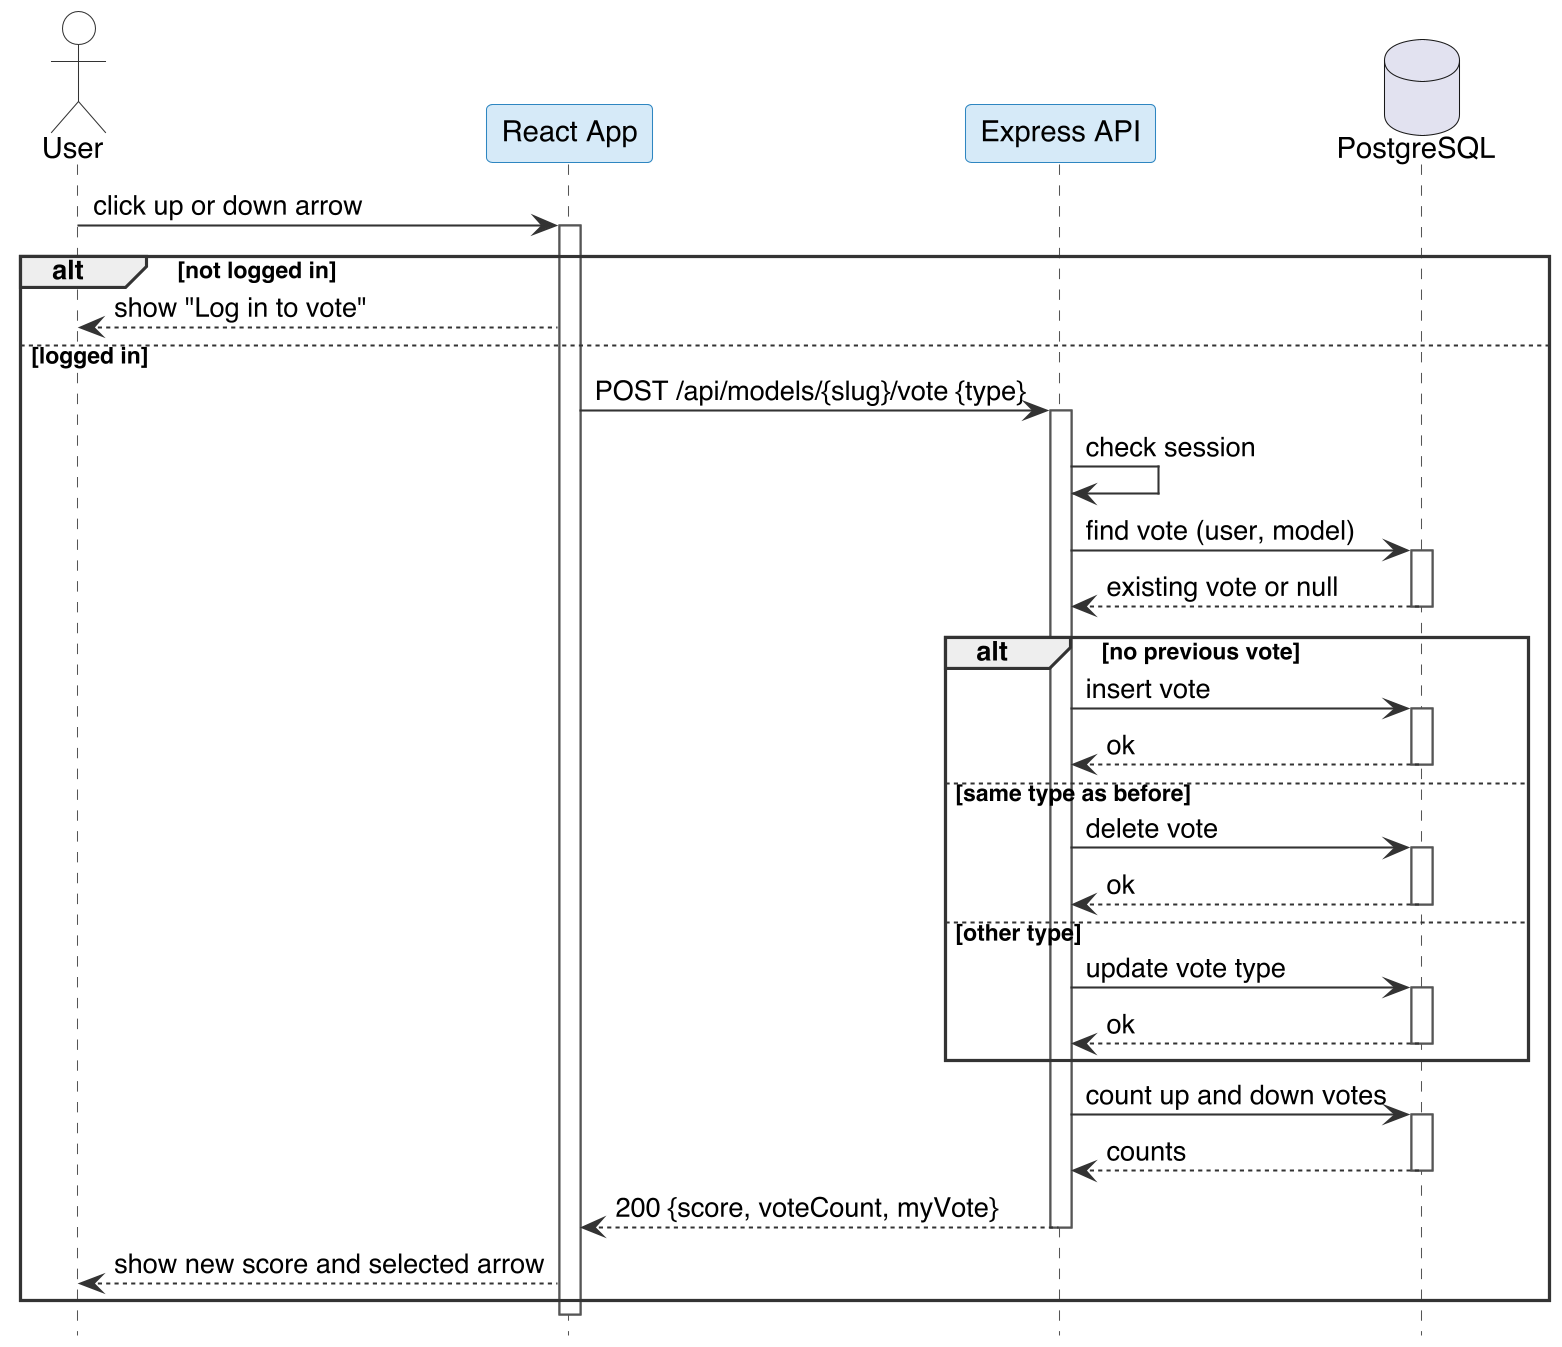
\includegraphics[width=\textwidth,height=0.6\textheight,keepaspectratio]{figures/vote-sequence.png}
  \caption{Sequence diagram of UC1 -- Voting for a model}
\end{figure}

\subsection{Use Case 2: Commenting on a Model}

\textbf{Actors:} Registered User, System

\textbf{Description:} the user writes a comment in the feed of a model to discuss its performance.

\textbf{Precondition:} the user is logged in and the account is active.

\textbf{Steps:}
\begin{enumerate}
  \item The user opens the page of a model.
  \item The user writes a comment and clicks on ``Send''.
  \item The system checks that the comment is not empty and has less than 1000 characters.
  \item The system saves the comment.
  \item The system shows the comment at the top of the feed.
\end{enumerate}

\textbf{Alternative flows:} if the user is not logged in, the system asks the user to log in. If the comment is empty or too long, the system shows an error and the user can correct it.

\begin{figure}[H]
  \centering
  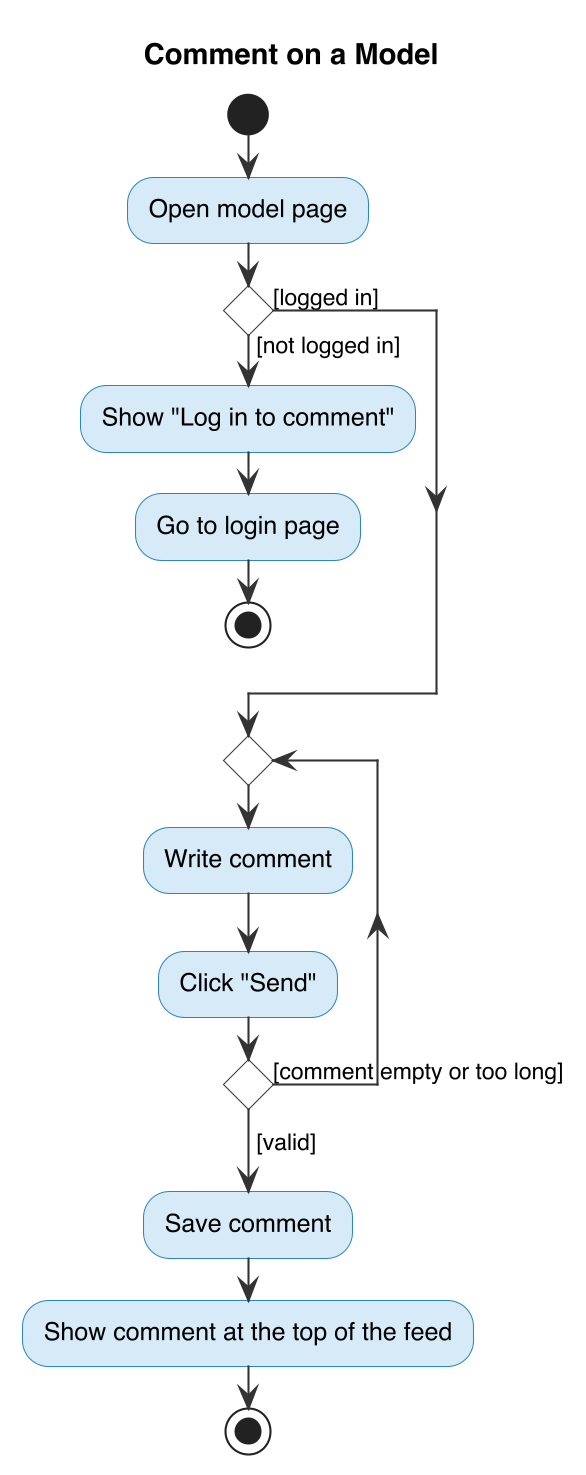
\includegraphics[width=\textwidth,height=0.6\textheight,keepaspectratio]{figures/comment-activity.png}
  \caption{Activity diagram of UC2 -- Commenting on a model}
\end{figure}

\section{Modeling Diagrams}

\subsection{Class Diagram}

The class diagram shows the main classes of the system, organized in five packages. \texttt{Vote} and \texttt{Score} are association classes: there is exactly one vote for each pair (user, model) and one score for each pair (model, benchmark). \texttt{Comment} is a normal class because a user can write many comments on the same model. The composition between \texttt{User} and \texttt{Comment} means that the comments are deleted with the account.

\begin{figure}[H]
  \centering
  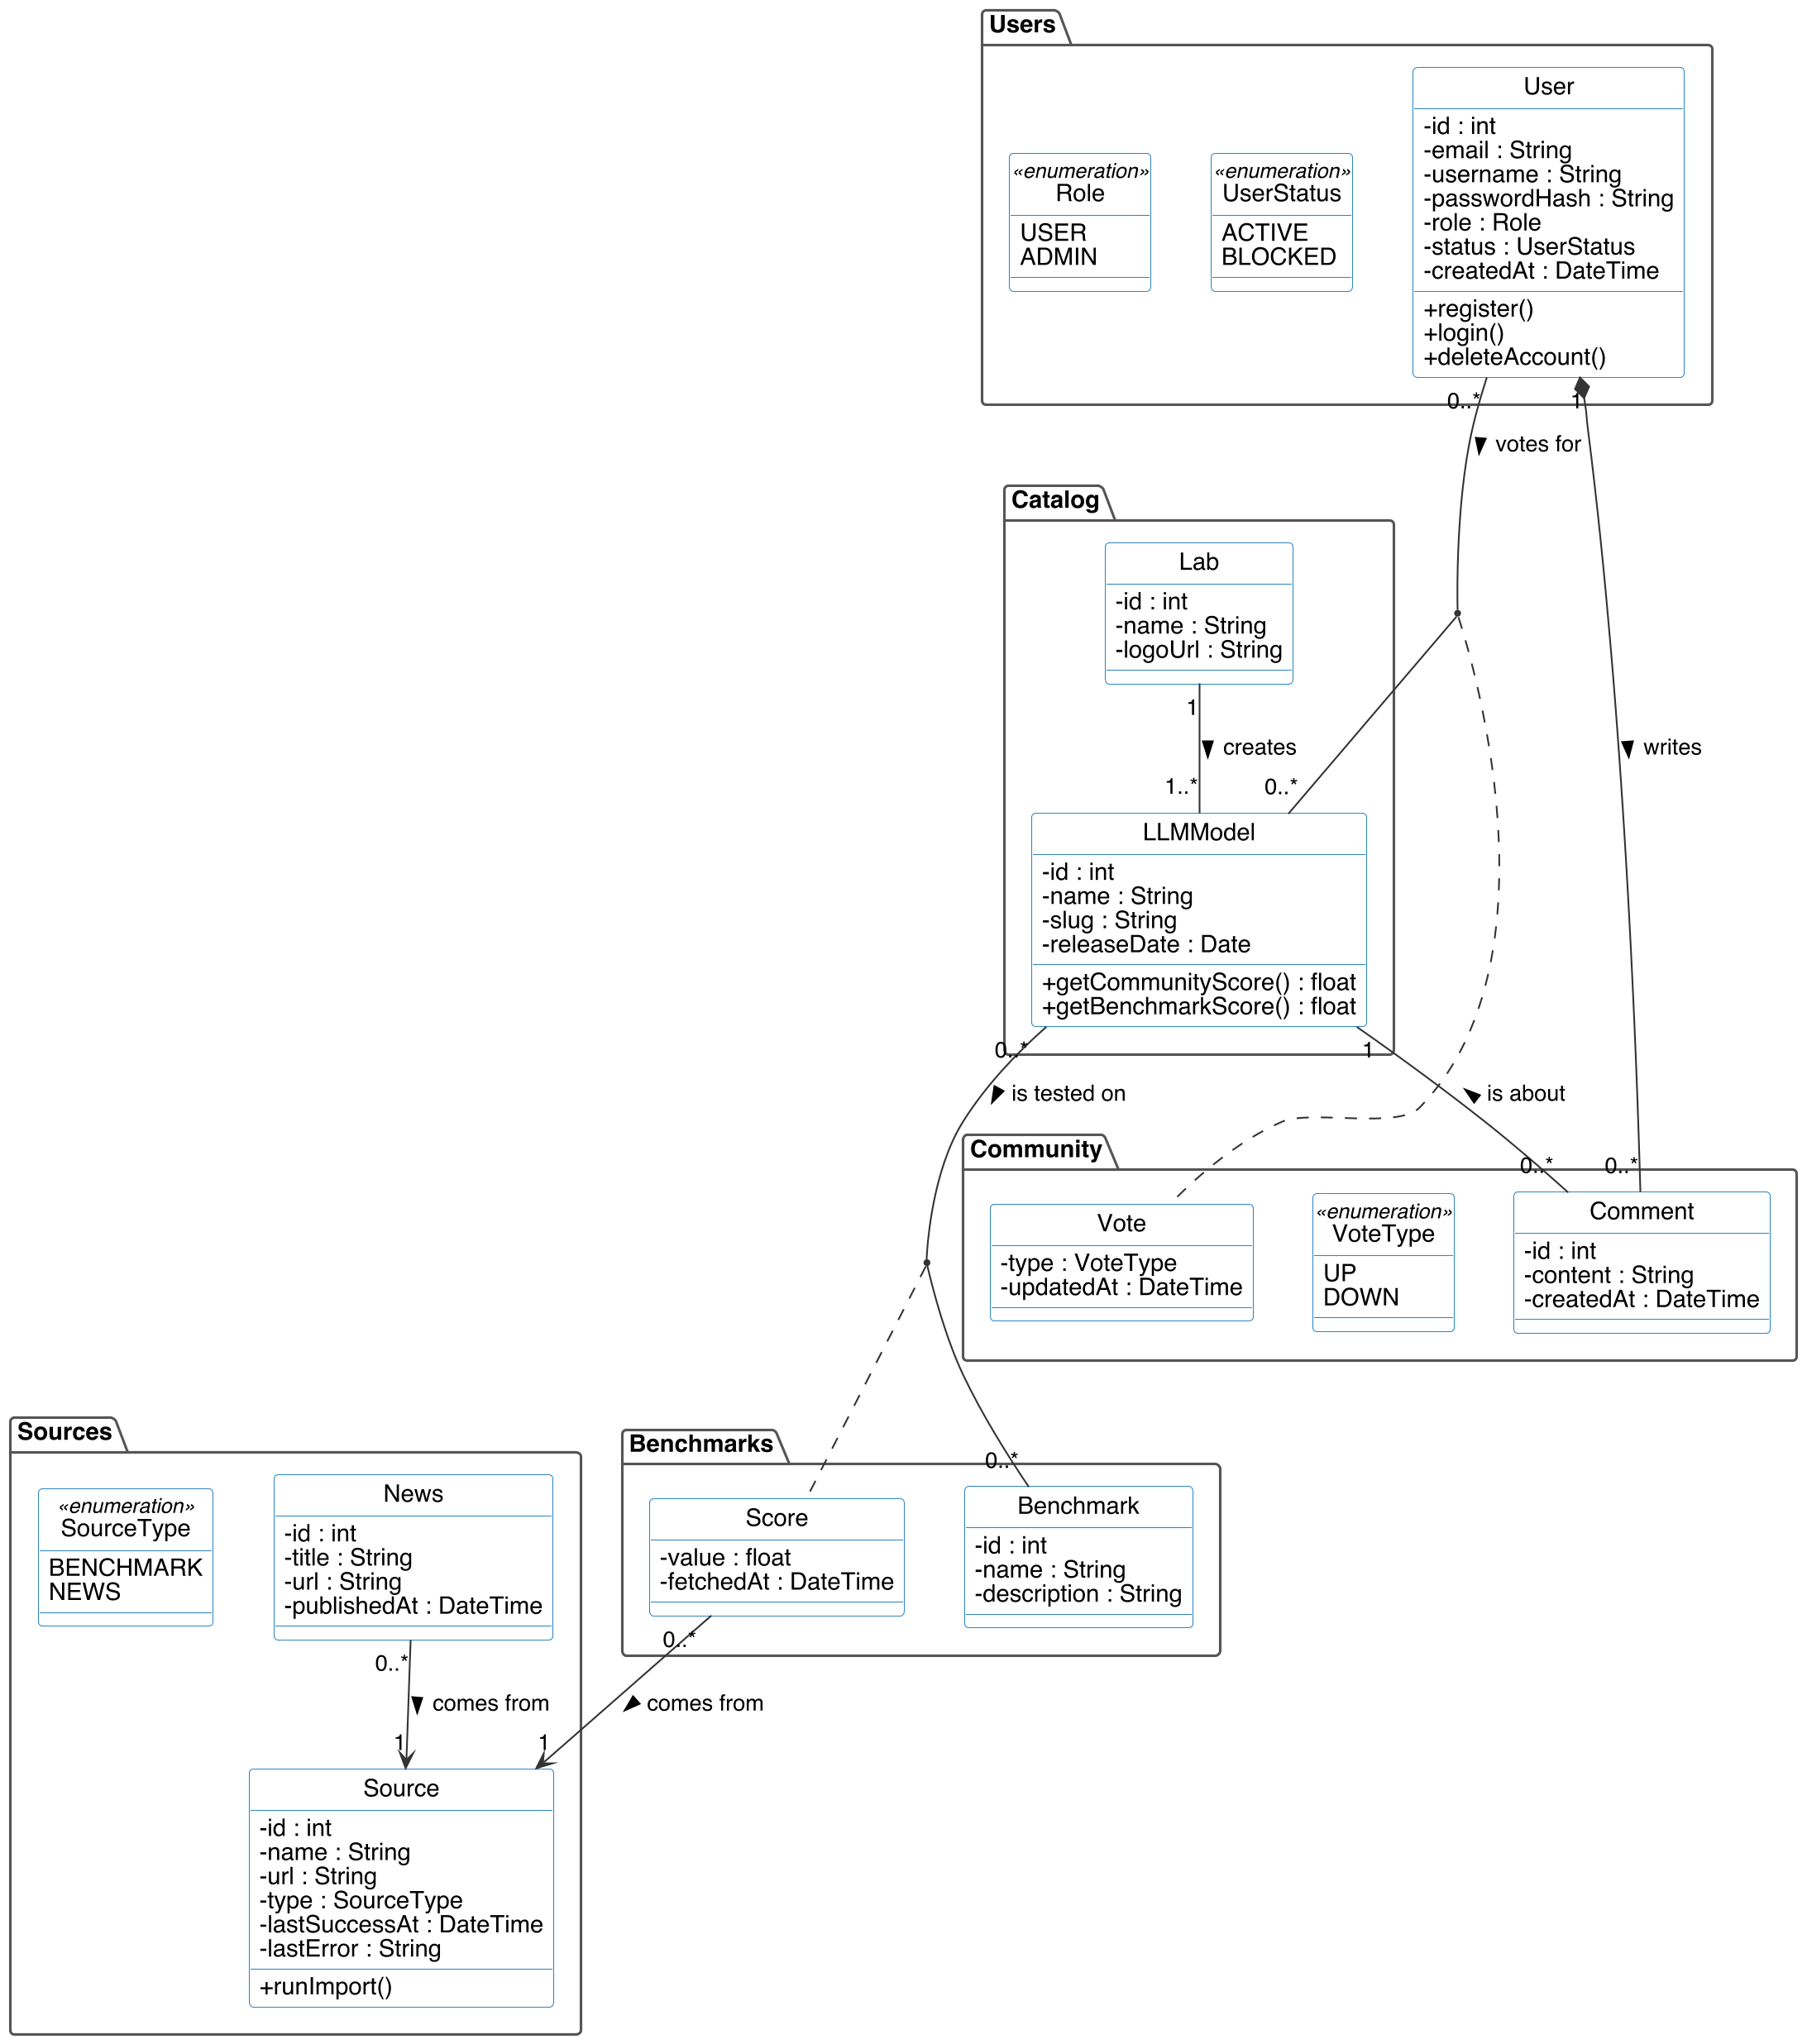
\includegraphics[width=\textwidth,height=0.75\textheight,keepaspectratio]{figures/class.png}
  \caption{Class diagram with packages}
\end{figure}

\subsection{Sequence Diagram}

This diagram shows how the model page is loaded, including the case where the model does not exist.

\begin{figure}[H]
  \centering
  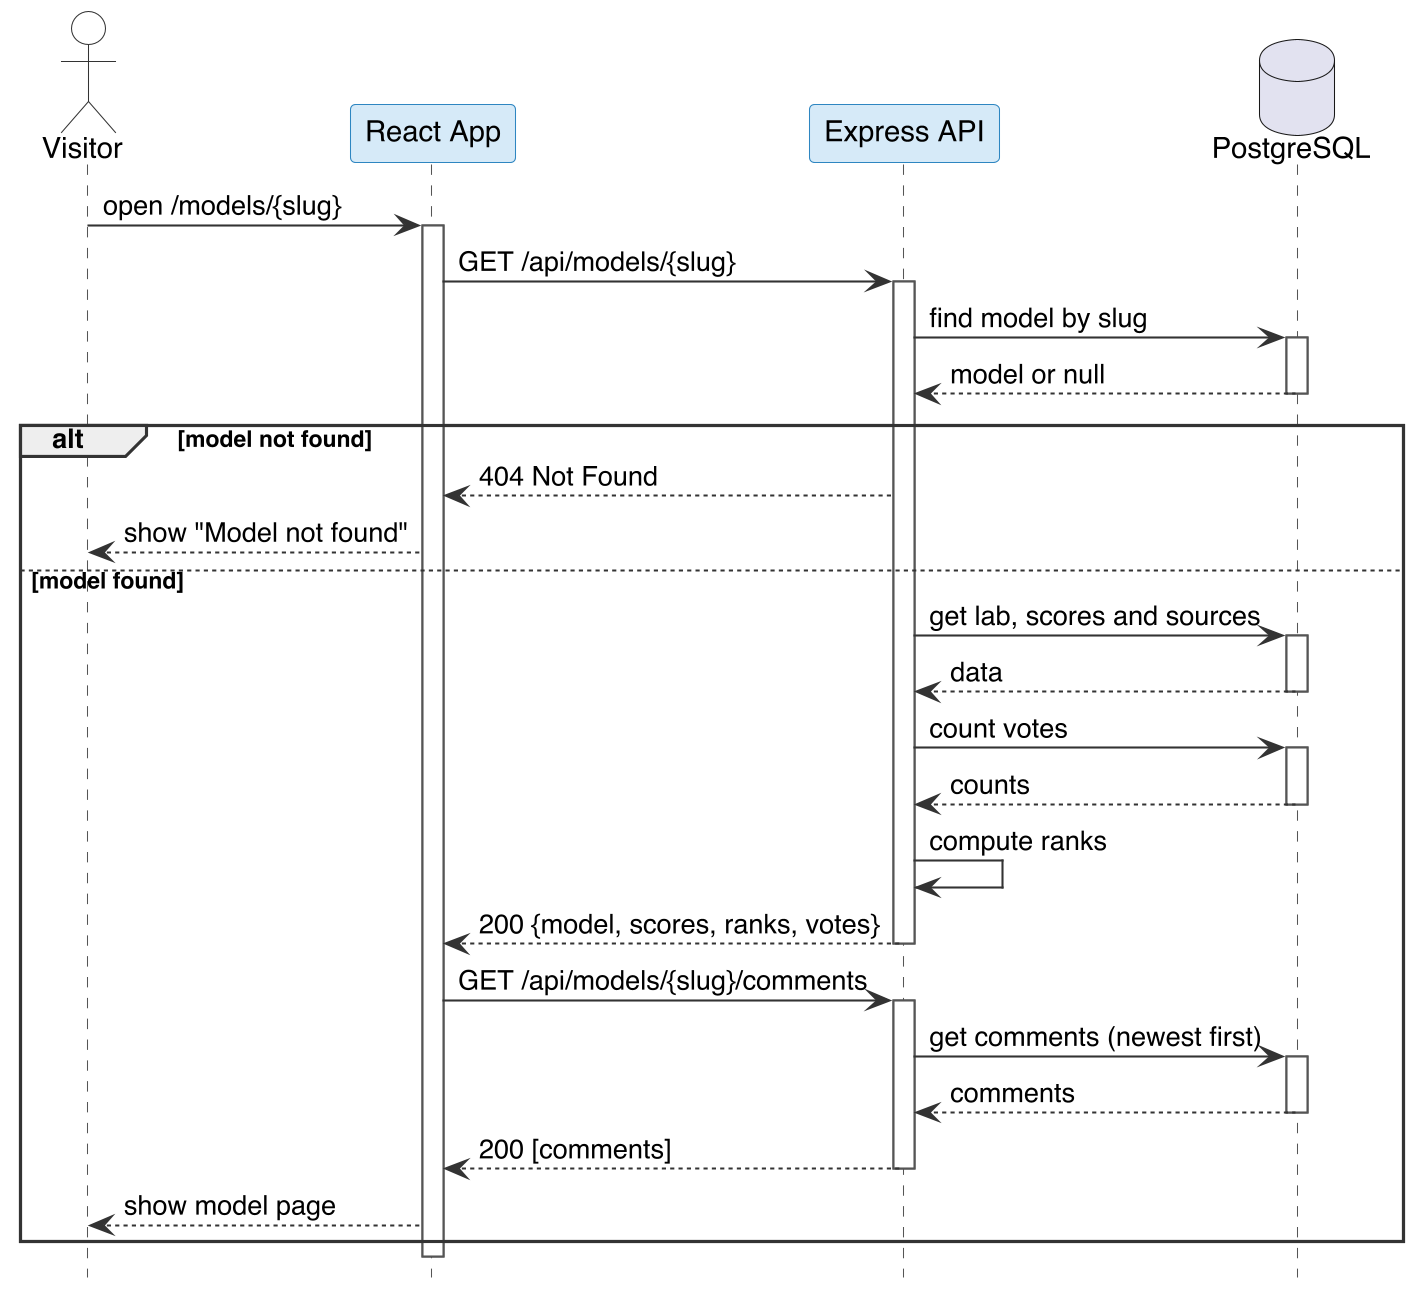
\includegraphics[width=\textwidth,height=0.6\textheight,keepaspectratio]{figures/model-page-sequence.png}
  \caption{Sequence diagram -- Opening a model page}
\end{figure}

\subsection{Use Case Diagram}

The Registered User inherits the use cases of the Visitor, and the Administrator inherits the use cases of the Registered User. Voting and commenting include logging in. ``Block author'' extends ``Delete any comment''.

\begin{figure}[H]
  \centering
  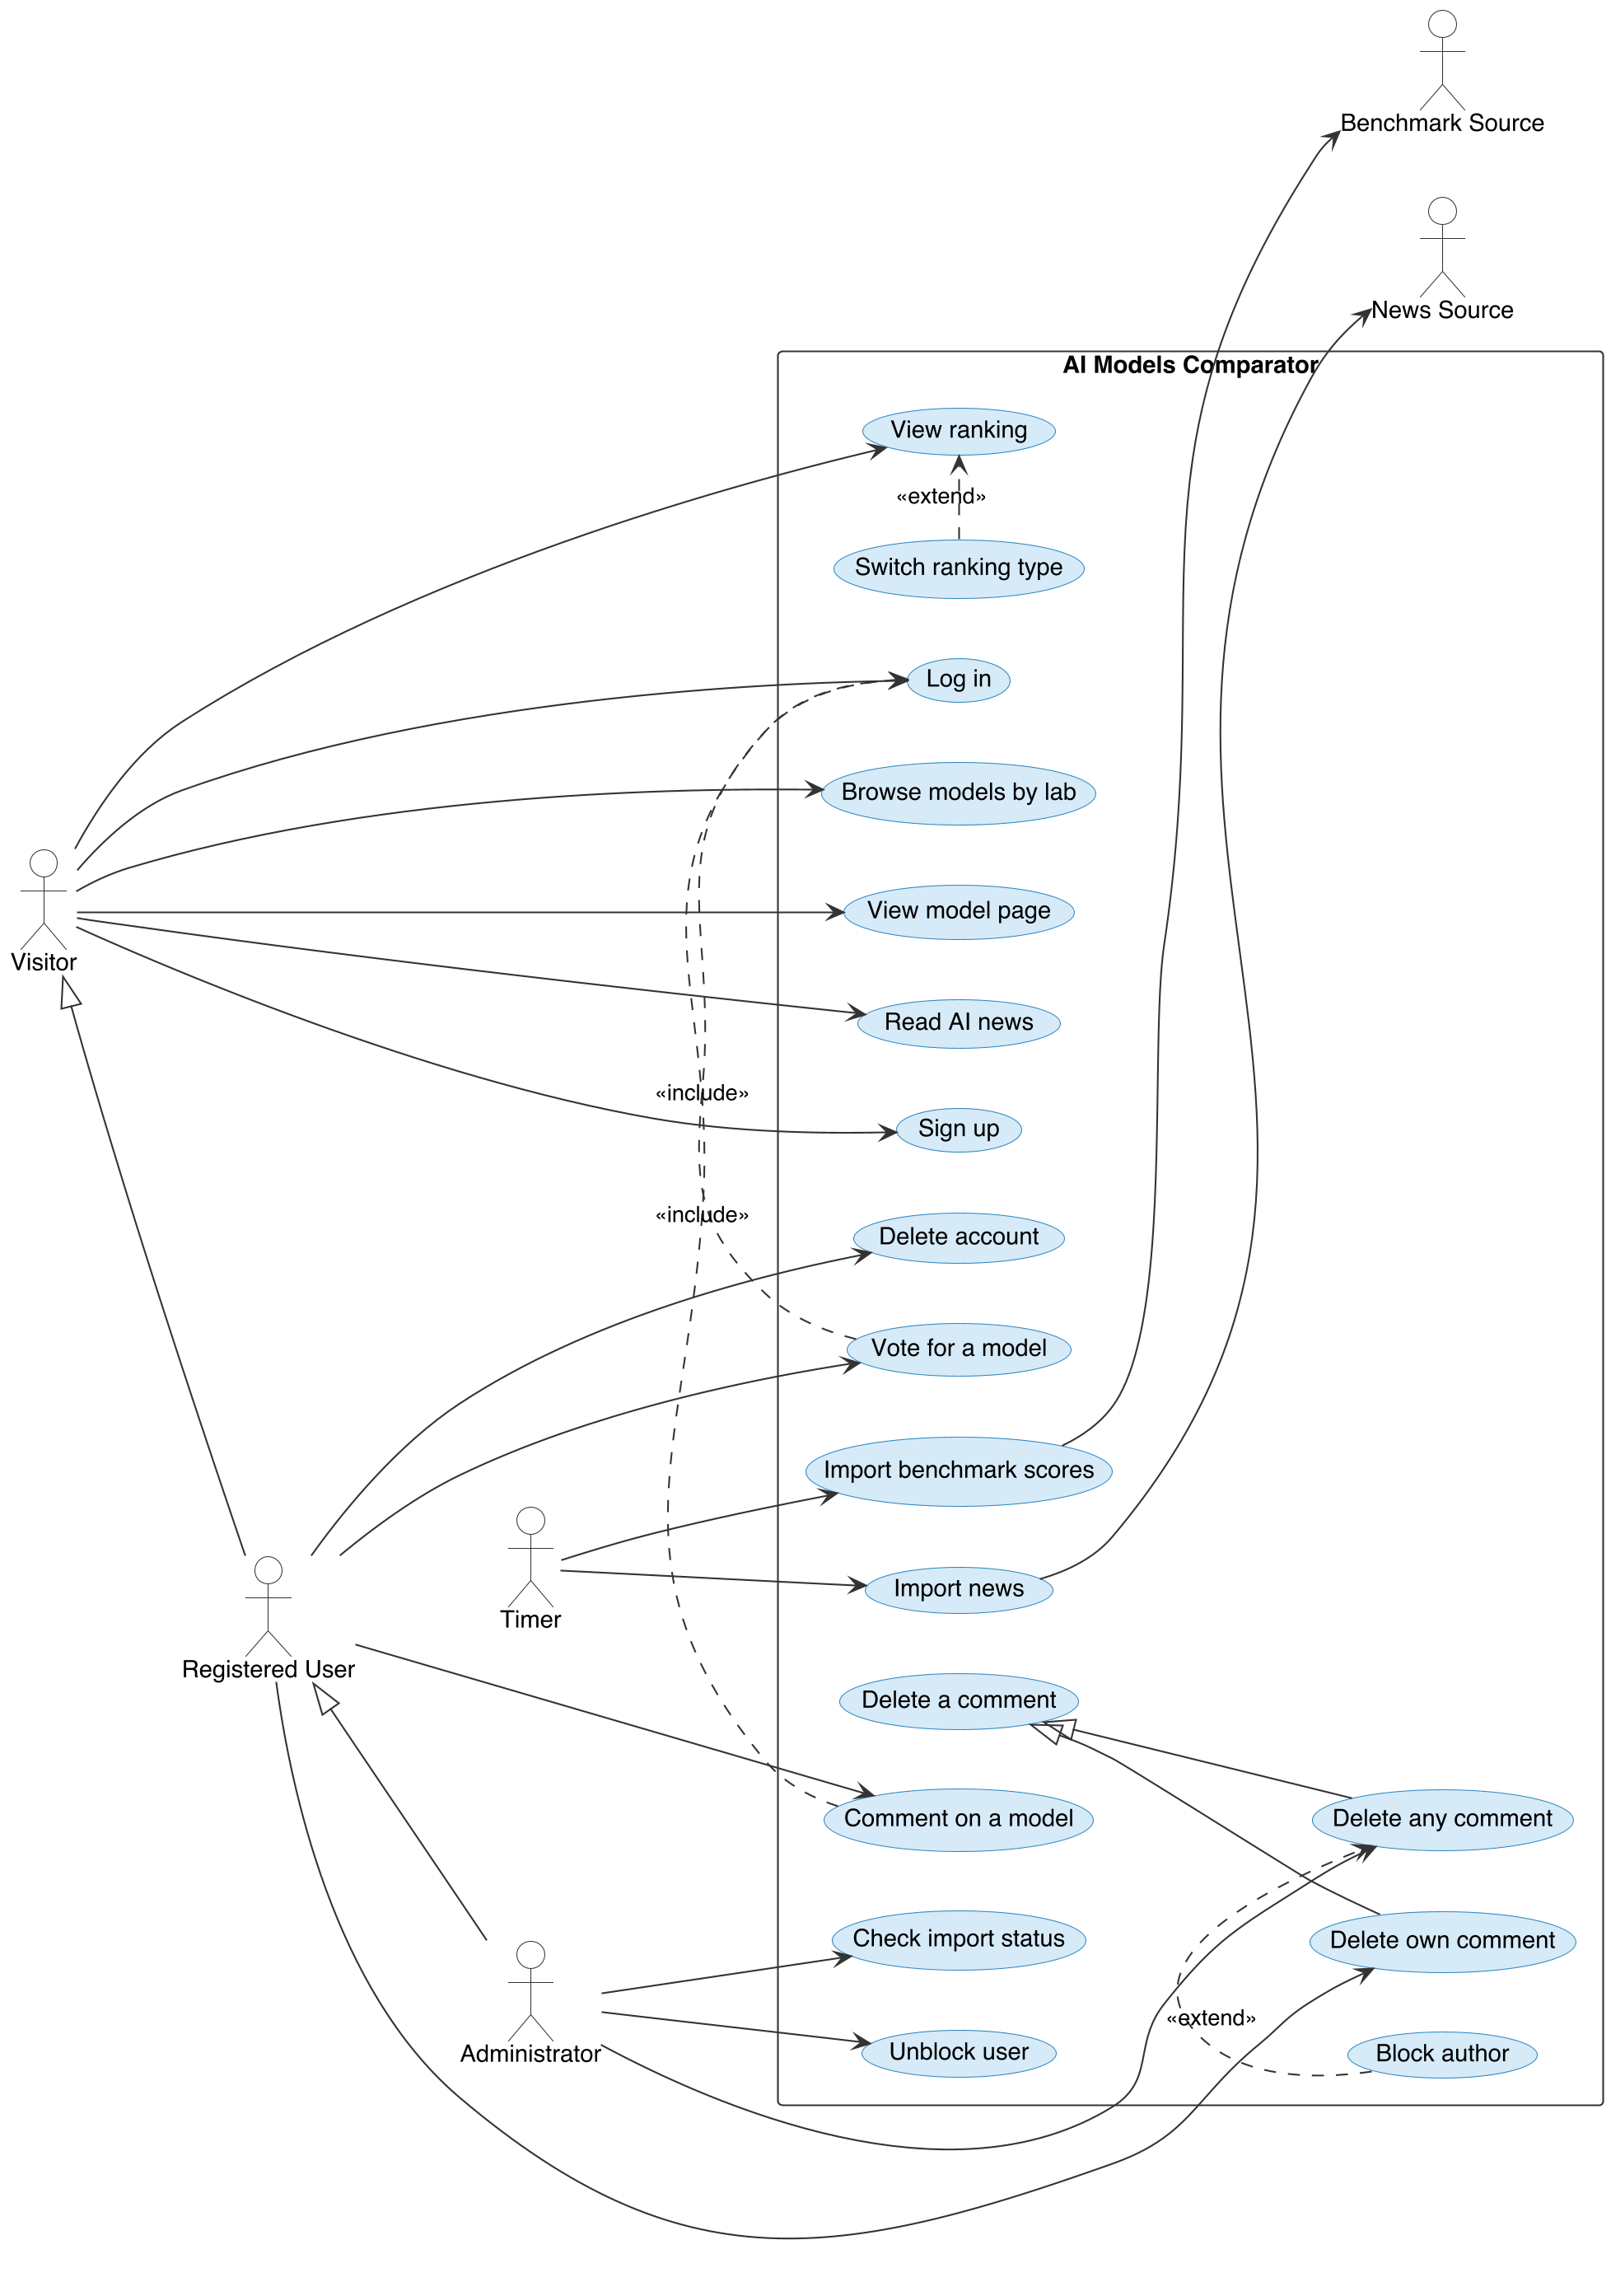
\includegraphics[width=\textwidth,height=0.75\textheight,keepaspectratio]{figures/usecase.png}
  \caption{Use case diagram}
\end{figure}

\section{External Interfaces}

\subsection{User Interface}

\begin{center}
\begin{tabularx}{\textwidth}{llX}
  \toprule
  \textbf{Route} & \textbf{Access} & \textbf{Content} \\
  \midrule
  \texttt{/} & Public & Title and three buttons: Models, Ranking, News \\
  \texttt{/login} & Public & Log in and Sign up tabs \\
  \texttt{/models} & Public & Labs with their logo, and their models (alphabetical order) \\
  \texttt{/models/\{slug\}} & Public & Model details, benchmarks, votes, comments \\
  \texttt{/ranking} & Public & Community or benchmark ranking, with the other rank on each line \\
  \texttt{/news} & Public & AI news, newest first \\
  \texttt{/account} & User & Username, email, ``Delete my account'' button \\
  \texttt{/admin} & Admin & Users, recent comments, import status \\
  \bottomrule
\end{tabularx}
\end{center}

\noindent\textbf{Wireframes} (the names and numbers are only examples):

\begin{figure}[H]
  \centering
  \begin{minipage}{0.48\textwidth}
    \centering
    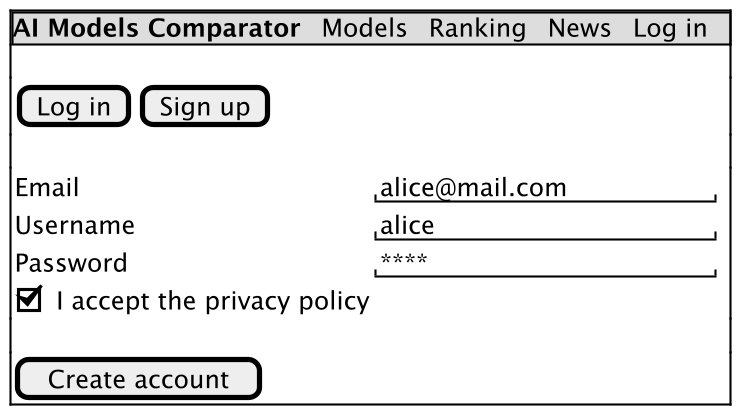
\includegraphics[width=\textwidth]{figures/wf-login.png}
    \caption{Login / Sign up}
  \end{minipage}\hfill
  \begin{minipage}{0.48\textwidth}
    \centering
    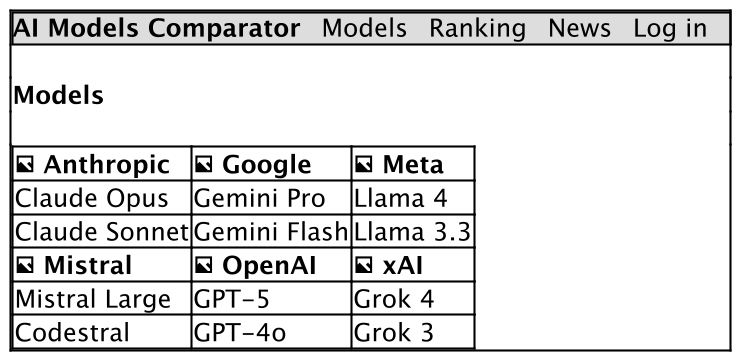
\includegraphics[width=\textwidth]{figures/wf-models.png}
    \caption{Models page}
  \end{minipage}
\end{figure}

\begin{figure}[H]
  \centering
  \begin{minipage}{0.48\textwidth}
    \centering
    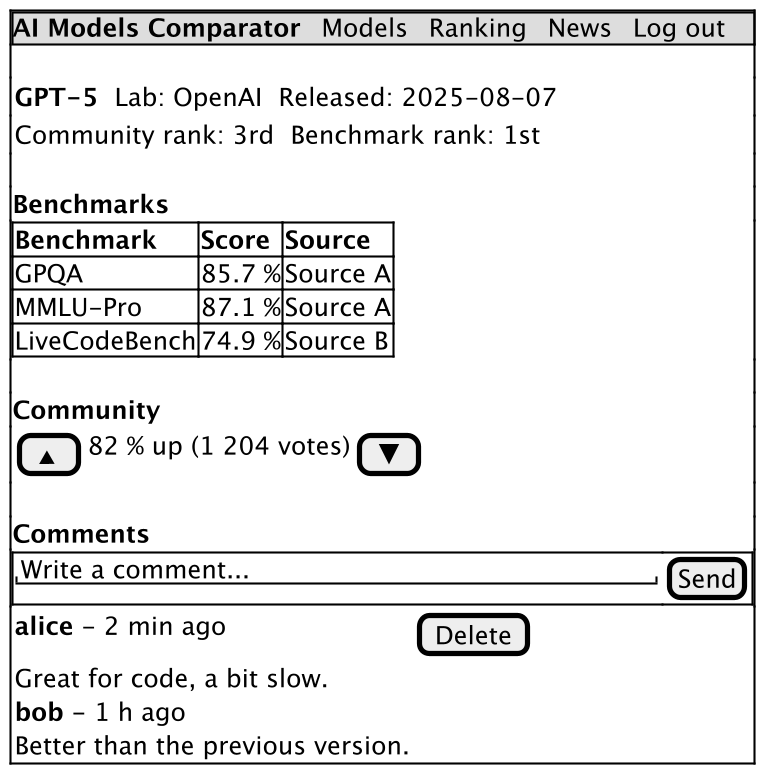
\includegraphics[width=\textwidth]{figures/wf-model-page.png}
    \caption{Model page}
  \end{minipage}\hfill
  \begin{minipage}{0.48\textwidth}
    \centering
    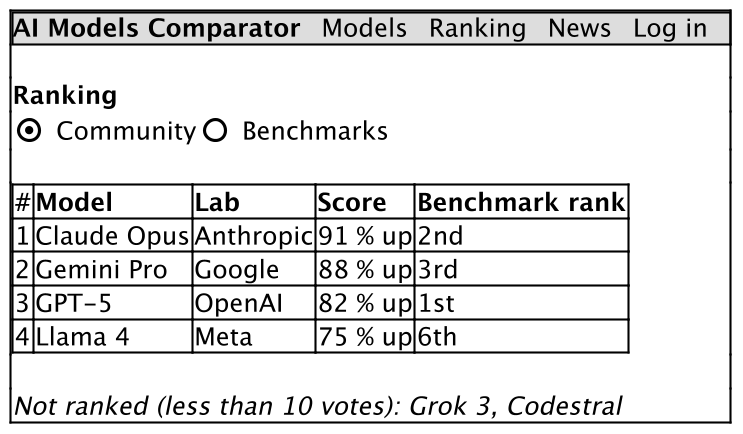
\includegraphics[width=\textwidth]{figures/wf-ranking.png}
    \caption{Ranking page}
  \end{minipage}
\end{figure}

\subsection{Hardware Interfaces}

The system does not use any special hardware. It works on any computer or phone with a web browser.

\subsection{Software Interfaces}

\begin{itemize}
  \item \textbf{Benchmark source API:} the backend calls a public API (REST, JSON) to get the benchmark scores.
  \item \textbf{AI news feed:} the backend reads a public RSS feed (XML) to get the news.
  \item \textbf{PostgreSQL:} the backend stores all the data in a PostgreSQL database.
\end{itemize}

\subsection{Communication Interfaces}

\begin{itemize}
  \item The frontend and the backend communicate with a REST API over HTTPS, using JSON.
  \item The user session is stored in a secure cookie (HttpOnly, Secure).
\end{itemize}

\section{Other Requirements}

\subsection{Security and Privacy}

\begin{itemize}
  \item We only store the email, the username and the hashed password of the users (GDPR data minimisation).
  \item The privacy policy is shown at sign up and must be accepted.
  \item When an account is deleted, all its personal data, votes and comments are deleted.
  \item The database is saved every day.
\end{itemize}

\subsection{Compatibility}

\begin{itemize}
  \item The website must work on the last two versions of Chrome, Firefox, Safari and Edge.
\end{itemize}

\subsection{Maintainability}

\begin{itemize}
  \item The code is split into modules (one service for each feature) so that a feature can change without breaking the others.
\end{itemize}

\section{Appendices}

\begin{itemize}
  \item \textbf{Appendix A:} wireframes of the main pages (Section 6.1).
  \item \textbf{Appendix B:} REST API documentation (see the SDD, Section 5).
\end{itemize}

\section{Index}

\begin{itemize}
  \item \textbf{Benchmark ranking:} 3.1.2
  \item \textbf{Comments:} 3.1.5, 4.2
  \item \textbf{Community ranking:} 3.1.3, 4.1
  \item \textbf{GDPR:} 2.4, 7.1
  \item \textbf{Vote:} 3.1.3, 4.1, 5.1
\end{itemize}

\end{document}
